\documentclass[a4paper, 11pt]{report}

\usepackage{shorttoc}
\usepackage{amsmath}
\usepackage{amssymb}
\usepackage{graphicx}

\begin{document}

\begin{titlepage}
    %--------------------------
    % Page de garde du rapport
    %--------------------------
    \parindent=0pt
    \hrulefill
    \begin{center}\bfseries\Huge
        Modeling of the shape of proteins from SAXS data
    \end{center}

    \hrulefill
    \vspace*{1cm}
    \begin{center}\bfseries\Large           %author
        Guillaume Bonamis
    \end{center}

    \begin{center}\bfseries\Large           %supervisor
        Supervisor: J\'er\^ome Kieffer
    \end{center}

    \vspace*{\stretch{2}}
    \begin{flushright}
        August 27, 2015
    \end{flushright}   
    
    %rajouter un mot sur le tuteur Lille1
\end{titlepage}


\chapter*{Acknowledgements}
\addcontentsline{toc}{chapter}{Acknowledgements}
\pagenumbering{Roman}
    %-------------------------------------
    % Page pour les divers remerciements
    %-------------------------------------


\tableofcontents
\addcontentsline{toc}{chapter}{Table of contents}
\pagenumbering{arabic}


\chapter{Introduction}
    %-------------------
    % Premier chapitre   
    %-------------------

\section{The European Synchrotron Radiation Facility}

The ESRF is a user facility providing very intense X-rays beams to scientists to
perform absorption, diffraction or spectroscopy experiments.
The X-rays in a synchrotron are generated by electrons travelling at 
99.9999\% of the speed of light, inside a long, circular tube in near-
perfect vacuum.\\

At the ESRF, these electrons are first accelerated by a 16-metre-long 
linear accelerator (linac) before entering a small, racetrack shaped 
booster accelerator. 
Once they have reached their final speed (at an energy level of 6 GeV), 
these high-energy electrons are injected into the vacuum tube of the
844-metre-long storage ring.
Here they are guided on their orbital path by magnets. 
In between these magnets, the electrons pass through insertion 
devices, also called undulators.
During each passage, the electrons release bursts of intense X-rays, 
along with electromagnetic radiation with other wavelengths, from 
infrared light to gamma-rays. 
These X-ray bursts are projected in the forward direction, like a 
laser beam thin as a human hair (0.1 mm diametre).\\

The synchrotron X-ray beam leaves the main storage ring at a point a 
few metres after the undulator. 
Undulators are placed at 30 positions around the storage ring.
Upon leaving the storage ring, the X-rays enter one of 41 beamlines, 
each an ensemble of laboratory blocks or “hutches” where the actual 
research takes place. 
The figure~\ref{fgr:synchrotron} sum this running.

\begin{figure}
\centering
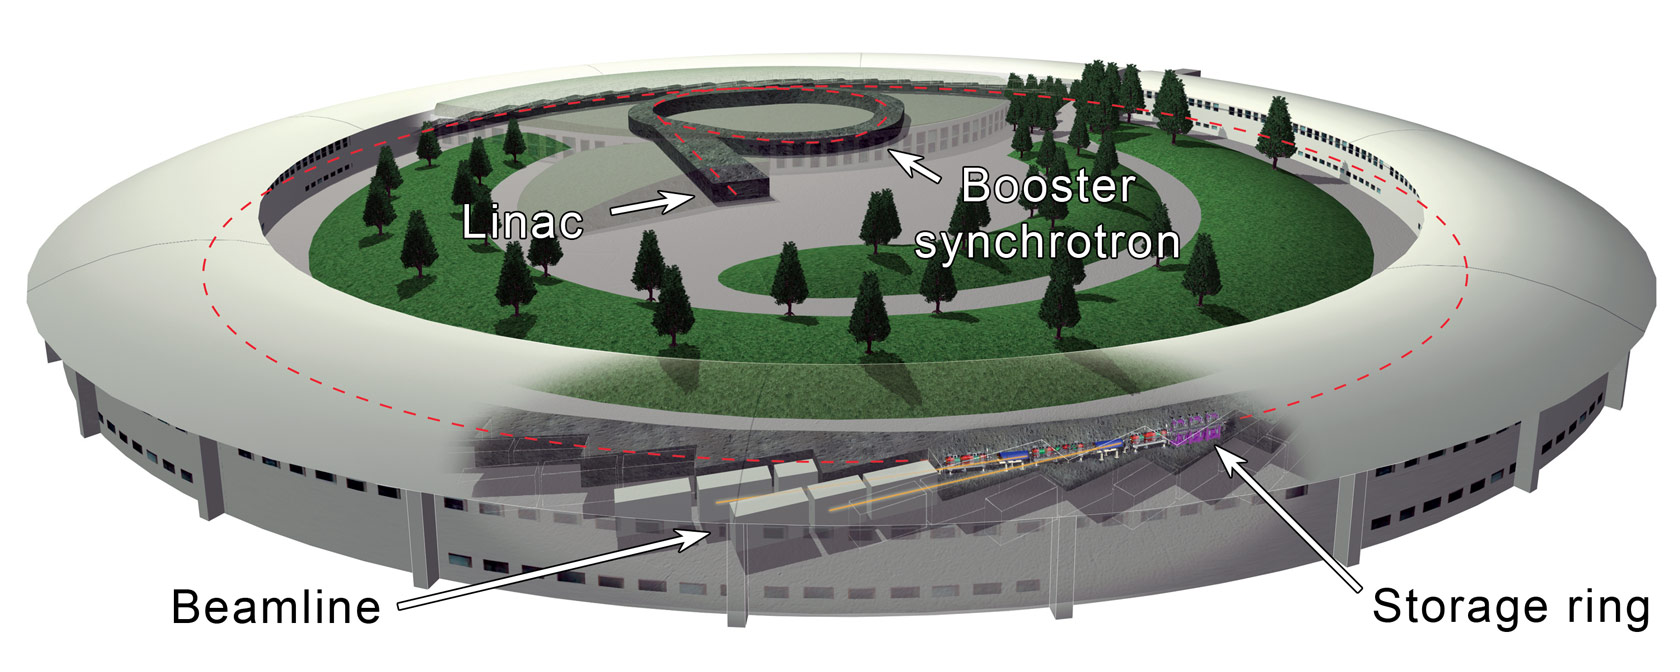
\includegraphics[scale=0.22]{synchrotron.png}
\caption{Chart of the ESRF with its main components, linac, booster, 
    storage ring and beamlines}
\label{fgr:synchrotron}
\end{figure}

\section{BioSAXS beamline BM29}
\label{bm29}
BM29 \cite{BM29paper} is a beamline for Small Angle X-ray Scattering 
(SAXS) experiments of biological macromolecule solutions with the goal 
to determine their 3-dimensional structures in a natural state with a 
'low' resolution (few nm). 
The beamline data acquisition running is based on a pipeline of 
individual tasks, highly automated, from the inputs to the final 
results. 
Here will be shortly described this series of process, focussing on 
what matter for our subject.
All data treatments have recently been described in \cite{BM29news} 
(submitted to \textit{Journal of Applied Crystallography}).\\

The series of tasks is controlled by EDNA, which is a plugin-based 
framework dedicated to pipelines data-analysis building \cite{edna}. 
It begin with the acquisition of the 2-d scattering image of the 
studied sample by a detector, a Pilatus 1M for BM29. 
Then, the global data-analysis process can be divided in four steps: 
\begin{itemize}
 \item azimuthal integration of the image
 \item background correction (scattering of the sample environment)
 \item basic analysis of the scattering curve
 \item ab-initio modelling
\end{itemize}

\begin{figure}
\centering
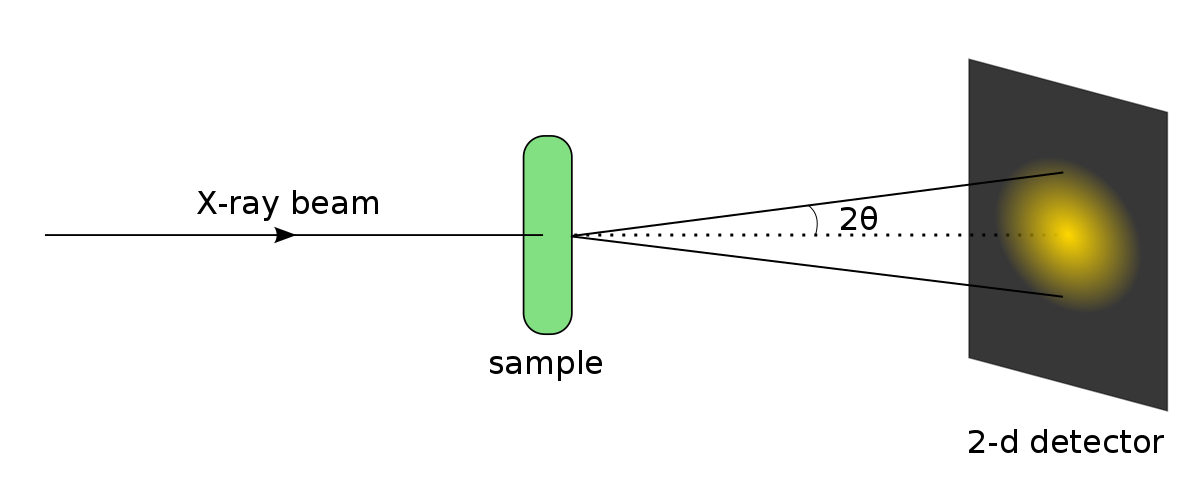
\includegraphics[scale=0.3]{schemaSAXS.png}
\caption{Schema of a SAXS experiment, scattering of the incident beam 
    create the scattered image on the detector}
\label{fgr:schemaSAXS}
\end{figure}

The image obtained represents the X-ray scattering by the sample, it 
has a cylindrical symmetry along the scattered beam, as seen on 
figure~\ref{fgr:schemaSAXS}. 
The first step consists in averaging the 2-d image along the 
symmetry axis (also called azimuthal integration).  
This operation is performed using FabIO \cite{fabio} for the image 
reading and PyFAI \cite{pyFAI} for the azimuthal integration and the 
result is a curve representing the scattered intensity function of the 
scattering vector $q = 4 \pi \frac{sin(\theta)}{\lambda}$ (expressed 
in inverse nanometers).

This curve has to be background-corrected: an EDNA plugin subtracts the
scattering intensity of the sample environment, recorded using a buffer
solution, to the sample curve, resulting in only the scattering signal of the
macromolecule. The background-corrected curve is then analysed with several
tools from the \textsc{atsas} package \cite{atsas}. 
The EDNA analysis pipeline generates automatically Guinier and Kratky
analysis plots for visual analysis of the scattering signal.\\

The fourth step of the data-analysis is the ab-initio modelling, 
presented in the following section, which is the core of the subject.

\section{Ab-initio modelling}
\label{modelling}                           %flag pour citer cette section

Ab-initio modelling aims at building a low-resolution 3-d  
model of the macromolecule of interest. 
For it, BM29 uses other tools from the \textsc{atsas} package as 
follow.\\

The first step of the modelling consists in reconstructing many ($N$, ususally 8
or 16) 3-d dummy-atoms models from the background-corrected curve with 
\textit{dammif} \cite{dammif}. 
These dummy-atoms models (DAM) are then selected according to two 
parameters computed with the curve: 
\[
R = \frac {\sum {||I_{obs}| - |I_{calc}||}}{\sum {|I_{obs}|}}; \ \ \ 
\chi^{2} = \sum {\frac {(I_{obs} - I_{calc})^{2}}{\sigma^{2}}}
\]
These two values allow to evaluate the goodness of the fit. 
The thresholds are respectively the mean plus one or two standard 
deviation, and models out of range are simply discarded.

Remaining DAM are then superimposed two by two using the \textit{supcomb}
\cite{supcomb} program which reports the Normalized Spatial
Discrepancy (NSD), a metric to evaluate the difference between two
models.
It allows the segregation of similar models and the others. 
So, once again, outlier models are discarded based on the NSD
values.
For each DAM, the mean of its NSD with others is computed; 
if this value exceeds the mean plus two time the standard 
deviation, it is discarded. 
The DAM with the lowest value is the reference model.\\

So here, at the moment of the process, $N - n$ models remain and one 
of them is the reference. 
All these $N - n$ models are merged with \textit{damaver} 
\cite{damaver}. 
Subsequently \textit{damfilt} gets the average DAM (which is not solution of
the problem) and \textit{damstart} generates an input model for 
\textit{dammin} \cite{dammin} which refines the model to fit the 
subtacted curve. 
The outcome of the Monte-Carlo refinement performed by \textit{dammin} is the
final model which can be interpreted by biologists (comparison with fragments
coming from NMR or comparison with other technics).

\section{Traineeship subject}

The topic of the traineeship was to work on the part "superimposition 
and selection of the models" of the modelling process. 
In fact, all the modelling process was pointed out as the most 
problematic according to the beamline scientists for several reason:
\begin{enumerate}
\item the BM29 pipeline is based on Python whereas most
of the \textsc{atsas} package is written in Fortran, so for a better 
integration in the pipeline, a Python library could be advantageous. 
\item programs from this package are closed source and 
changing from version to version add difficulties for their 
integration in the pipeline. 
\item the execution time of these programs make the ab-initio modelling the
bottleneck of the BM29 pipeline. 
\item sometimes the whole EDNA pipeline needs to be aborted 
due to \textit{dammin}, not returning after half an hour.
\end{enumerate}

In accordance with these observations, it was decided to create a 
homemade package to overpass these data-analysis problems. 
These package has been called FreeSAS, is open source and free (under 
the MIT License). 
Written in Python, it aims at providing tools for the BioSAXS data 
analysis, with an execution time optimized and providing reliable 
results. 
The subject was dedicated to this Python package, and especially the 
re-implementation of the superimposition of the DAM (so previously 
done by \textit{supcomb}) and the selection of those to keep along the 
process.\\
In the following chapter, we will describe all the implementation 
computed, and the theory behind them, to reach our aim. 
Then, in chapter 3, we will present an usage of FreeSAS using the 
scattering curve obtained from a protein called Lysozyme.


\chapter{FreeSAS implementation}
    %--------------------
    % Deuxieme chapitre  
    %--------------------

As mentioned previously, FreeSAS is a Python package for BioSAXS data-
analysis. 
It is built of several modules, each focusing on a special task. 
We will describe in this chapter, for each module of FreeSAS:
\begin{itemize}
 \item the tasks needed to be executed
 \item the physical theory behind this task and its usefulness in our 
       global process
 \item the different Python tools and algorithms used in the module to 
       execute this task
\end{itemize}
The last section will describe the way all these tasks are exploited 
to create a "global process" computing the wanted result. 

\section{Reading inputs data}

The library has to be able to work within the BM29 pipeline presented 
in section \ref{bm29} and used in production for a few years  now. 
As a component of a larger piece of software, it has to deal with inputs 
coming from other software, especially the \textsc{atsas} programs used
upstream and needs to provide outputs compatible with \textsc{atsas}, also used
downstream.
Here we will focus on the reading of the input structures and describe the
ones we are interested in.

The inputs of the superimposition module is the
outputs DAM of the various \textit{dammif} runs. 
These structures are written in files using the PDB format (for 
Protein Data Bank) \cite{pdb}, a standard representation of 
macromolecular structure data.\\
The (simplistic) parser written copes for two things: reading the atoms'
coordinates (beads) and retriving the quality of the fit of the model on the
experimental data ($\chi^2$ and $R$-value).
Those numbers represent the quality of the model, calculated using the 
difference between the actual SAXS curve and the simulated one from the
corresponding model. 
Those goodness of fit values are only used to reject model badly fitting
experimental data.

The second piece of information to retrieve is the dummy-atoms coordinates. 
As already mentioned, only low-resolution information are available in SAXS data 
hence the structure of model is made of dummy-atoms.
They are not actual atoms, but indicate there is 
some material (the macromolecule) at their positions, and where there is
no dummy-atoms, it is solvent. 
Typical DAM used in this project had 500 dummy-atoms (order of magnitude).
The parser written was dedicated to these task: to read the pdb file 
to select the data we needed, and then to keep in memory in one hand 
the $R-value$ of the DAM and in an other hand the Cartesian coordinates (x, y, 
z, in Angstrom) of each dummy-atoms of the model. 
These coordinates are stored as a 2-d numpy array from the 
\textit{NumPy} package for scientific Python \cite{numpy}; they are 
necessary for geometric handling we will have to do along our process.

\section{Similarity calculation}

To be able to merge similar models, and reject dis-similar ones,
one needs to define the similarity of two models. 
This section introduces a ``distance'' to measure this  
similarity and describes its implemention in the FreeSAS
package.

The likeness of two 3-d models can be, at first glance, very 
subjective. 
To be able to compute it, we use a metric called Normalized Spatial 
Discrepancy (NSD), introduced by Kozin and Svergun in their paper 
\textit{Automated matching of high- and low-resolution structural 
models} \cite{supcomb}. 
This value quantifies the dissimilarity between two sets of 
point $S_{1}$ and $S_{2}$, in our case in a three-dimensionnal space.
Those sets are neither ordered nor of same size ($N_{1}$ points for
$S_{1}$ and $N_{2}$ points for
$S_{2}$), making useless other techniques like Kabsch method
\cite{kabsch1976}.
The NSD has been built has an analogue to the standard Euclidian distance,
but as it is normalized, it is not homogeneous to a distance:

The NSD is introduced with the following formula:\\
\[
\rho(S_{1},S_{2})= \frac{1}{2} \sqrt {\frac{1}{N_{1}d_{2}^2} 
\cdot \sum\limits_{i=1}^{N_{1}} \rho^2(s_{1i}, S_{2}) + \frac{1}{N_{2}d_{1}^2} \cdot \sum\limits_{i=1}^{N_{2}} \rho^2(s_{2i}, S_{1})}
\]

For a point $s_{1i}$ in $S_{1}$, the Euclidian distance with all the 
points of $S_{2}$ is computed, and the minimal one is denoted as 
$\rho(s_{1i}, S_{2})$. 
The last parameters present in the formula is the fineness $d_{i}$. 
It correspond to the average Euclidian distance between a point of 
$S_{i}$ and its nearest neighbour.\\
The NSD can be used to measure the similarity of two sets of points as:
\begin{itemize}
 \item it is symmetric, $\rho(S_{1},S_{2}) = \rho(S_{2},S_{1})$
 \item it is stable, $\rho(S_{1},S_{2})$ function has a stable minimum
 \item $\rho(S_{1},S_{2}) = 0$ only if $S_{1} = S_{2}$
\end{itemize}

As the calculation of the NSD is the core of our process, it is of prime  
importance to optimize its implementation. This has been optimized in 3
subsequent steps (and supervised by careful profiling):
\begin{enumerate}
  \item numpy implementation calculating the 2d table of distances from all
  atoms in $S_{1}$ to any atoms in $S_{2}$, performing subsequently the minimum
  search in each row and column.
  \item Cython implementation \cite{cython} (a kind of Python code translated
  to C) which performs simulatneously the two minimum search (along row and
  column) for each pair of atoms, preventing a large 2d array allocation.
  \item An OpenMP \cite{openmp} implementation of the Cython version taking
  benefit of the multi-core systems available on modern computers.
\end{enumerate}

\section{Coarse superimposition of models}

The DAM, as generated by \textit{dammif}, are randomly oriented, so the NSD
between two models is not representative of their similarity.
That is why we have to first superimpose the models, using translation, rotation
and symmetries, so that the NSD only point out the dissimilarity.\\

The strategy implemented to superimpose two DAM (sets of
dummy-atoms $S_{1}$ and $S_{2}$) is similar to the one described in 
Kozin and Svergun's publication \cite{supcomb} and goes via a three-
steps process to bring them in their cannonical position:
\begin{itemize}
  \item the center of mass of the model is at the origin of the 
        coordinates axis (canonical translation)
  \item the principle axis of inertia of the model are aligned with 
        the coordinates axis (canonical rotation)
\end{itemize}
The last step consists in applying a special symmetry to $S_{2}$ to 
select the enantiomorph of $S_{2}$ corresponding on the one of $S_{1}$ 
(enantiomorph selection).

\subsection{Canonical translation}

The first stage consists in superimposing both models center of mass 
(COM). 
In the dummy-atoms modelization, all the dummy-atoms has the same mass 
so the COM coordinates of the model $k$ are computed as follow:
\[
x_{k}^0 = \frac{1}{N_{k}} \cdot \sum\limits_{i=1}^{N_{k}} x_{ik};\ \ \ 
y_{k}^0 = \frac{1}{N_{k}} \cdot \sum\limits_{i=1}^{N_{k}} y_{ik};\ \ \ 
z_{k}^0 = \frac{1}{N_{k}} \cdot \sum\limits_{i=1}^{N_{k}} z_{ik}
\]\\
From it, the translation to send the model $S_{k}$ to the coordinates' 
origin is calculated as $T_{k}^0 = (-x_{k}^0,\ -y_{k}^0,\ -z_{k}^0)$. 
Thus, the canonical translation of $S_{k}$ is $T_{k}^0$.

\subsection{Canonical rotation}

Next come the alignment stage. 
To compute the canonical rotation matrix of $S_{k}$, which will align 
principle axis of inertia of $S_{k}$ with the coordinates' axis, we 
first need to know its inertia matrix. 
It has to be compute with the COM of $S_{k}$ at the coordinates origin. 
It is given by:
\[
I_{k}=
\begin{pmatrix}
 I_{11} & I_{12} & I_{13} \\
 I_{21} & I_{22} & I_{23} \\
 I_{31} & I_{32} & I_{33} \\
\end{pmatrix}
\]\\
and knowing that each point of the set $S_{k}$ is defined by
$
s_{kq}=
\begin{pmatrix}
 x_{kq}^1 \\
 x_{kq}^2 \\
 x_{kq}^3 \\
\end{pmatrix}
$\\
we have
\[
I_{ij} = \frac{1}{N_{k}} \cdot \sum\limits_{q=1}^{N_{k}} 
[\delta_{ij} \cdot \sum\limits_{l=1}^3 
 (x_{kq}^l - {x_{kq}^l}^0)^2 -  (x_{kq}^i - {x_{kq}^i}^0) 
 \cdot (x_{kq}^j - {x_{kq}^j}^0)]
\]\\
It appears that $I_{k}$ tensor is symmetric real so we know that it 
can be diagonalized; we can compute its three eigenvalues 
$\lambda_{k1} \geq \lambda_{k2} \geq \lambda_{k3}$ and the three 
eigenvectors corresponding $v_{k1},\ v_{k2},\ v_{k3}$. 
We can create a rotation matrix compound by the columns from 
eigenvectors of $I_{k}$, sorted with rising order of associated 
eigenvalues. 
If this matrix is wrote $M_{k}$, is transposed $[M_{k}]^T$ is the 
rotation matrix which align $S_{k}$ axis of inertia with the 
coordinates axis \cite{supcomb}, the one we are looking for.

\subsection{Enantiomorph selection}

Before to be able to superimpose correctly $S_{2}$ on $S_{1}$, we need 
to take into account enantiomorphs. 
In fact, two enantiomorphs of a macromolecule generate the same SAXS 
curve, so that this method do not allows to segregate them. 
Thus, we do not make a difference for our data-analysis between two 
enantiomorphs; and it needs to be implemented. 
As we superimpose $S_{2}$ on $S_{1}$, we will force $S_{2}$ to be in 
the same enantiomorphic form that $S_{1}$. 
For it, we have to set $S_{1}$ and $S_{2}$ in their canonical 
position, so apply to them the transformation 
$[M_{k}]^T \times T_{k}^0$ corresponding.

Eight transformations are then performed on $S_{2}$ which correspond 
to the eight possible symmetries, four for each enantiomorph. 
Transformation matrices are as follow:
\[
\begin{pmatrix}
 \pm 1 & 0 & 0 & 0 \\
 0 & \pm 1 & 0 & 0 \\
 0 & 0 & \pm 1 & 0 \\
 0 & 0 & 0 & 1
\end{pmatrix}
\]\\
And after each transformation, the NSD between $S_{1}$ and $S_{2}$ is 
computed. 
The one minimizing the NSD is kept as the good symmetry for the 
following steps. 
The rotation matrix for $S_{2}$ is now the previous one $[M_{2}]^T$ 
multiplied by the symmetry matrix, we will write it $R_{2}$.\\

Finally, we are able to compute, for a set of dummy-atoms $S_{k}$, the 
canonical translation and rotation matrices. 
We now also the the transformation to apply to force a DAM to be in 
the same enantiomorphic form that an other one. 
To canonically superimpose two DAM we can apply on them the required 
transformation, but we chose to always align the second DAM on the 
first one initial position (to save execution time).\\
Thus, we apply the following transformation to $S_{2}$:
\[(T_{1}^0)^{-1} \times M_{1} \times R_{2} \times T_{2}^0\]

At the end of this process, we have two DAM whose centers of mass and 
principles axis of inertia are superimposed; we will say canonically 
superimposed. 

\section{Refined superimposition}

The canonical superimposition presented before produce a good fit of 
the two models (if they are similar), but it remains a coarse 
alignment we need to optimize for a better understanding of the 
dissimilarity between two DAM. 
The core of the superimposition process remains the same, we will add 
on it the following refinement algorithm.\\
 
We have to optimize the transformation applied to $S_{2}$ to align it 
with $S_{1}$, and the criterion of improvement will be the NSD, which 
has to be as low as possible. 
For it, we use the simplex optimizer provided by the \textit{SciPy} 
library \cite{scipy}. 
But to use it, accurate numerical parameters are needed. 
What we did is to extract from the global transformation matrix 
presented before six transformation parameters: 
$(x_{0}, y_{0}, z_{0})$, 
corresponding to the total translation applied to $S_{2}$, and 
$(\alpha, \beta, \gamma)$, 
which are the Euler angles extracted from the total rotation. 
The optimizer receives this six parameters and call a function which 
returns the NSD between $S_{1}$ and $S_{2}$ after the input 
transformation has been applied to $S_{2}$. 
This call is repeat again and again, refining each time the six 
parameters values to minimize the NSD returned.\\
When these iterations reach a landing, the optimizer is stopped and 
returns the six refined parameters and the minimized NSD. 
Here, the superimposition of the two models is optimized, the final 
NSD value is assumed to reflect the actual dissimilarity between them.\\

\section{Dummy atoms models selection}

The algorithm to superimpose two DAM has been fully described, it has 
to be implemented in order to superimpose the $N$ models outgoing of 
\textit{dammif}. \\

For it, dammif pdb files are first read with the FreeSAS parser and 
usefull data are extracted as presented before. 
Some properties we introduced are then computed from it. 
At this stage we dispose of $N$ detailled DAM and all we need to 
superimpose them.\\
The superimposition is implemented to obtain a NSD table $N*N$ sized. 
Each model is represented by one row and one column. 
Each bow in the table will contain the optimized NSD between the "row" 
model and the "column" model. 
To resume, we want a $N*N$ table with 
\[
table_{ij}=NSD(S_{i},S_{j})
\]\\ 
We know that all we will have zeros on the diagonal and the table will 
be symmetric because of two properties of the NSD:
\[
NSD(S_{i},S_{i})=0.00 \Rightarrow table_{ii}=0.00
\]
\[
NSD(S_{i},S_{j}) = NSD(S_{j},S_{i}) \Rightarrow table_{ij}=table_{ji}
\]\\
Thus we can compute $\frac{N \cdot (N-1)}{2}$ optimized 
superimpositions instead of $N*N$.\\

Once the NSD table generated, we dispose of all we need to select the 
dummy-atoms models.\\
The first criteria of selection have already been presented in 
\ref{modelling} section: the $\chi^2$ and the $R-value$. 
These two parameters are not dependent of the DAM position, they are 
computed before any movements. 
So for a gain of execution time, the test on them are computed before 
the superimposition process. 
Thus some models (say $x$) are discarded before to be superimposition, 
which allow us to skip the optimized alignment calculation to save 
time: $\frac{(N-x) \cdot (N-x-1)}{2}$ instead of 
$\frac{N \cdot (N-1)}{2}$.\\
The following criterion of selection has also been explained in 
\ref{modelling} section, the average NSD between each models and 
others. 
This variable is computed using the NSD table obtained by the process 
we know and the test is performed for each DAM remaining ($N-x$ at 
this level). 
A new series of models is discarded (or neither), that give us the 
$N-n$ acceptable DAM to follow the modelling process of EDNA. 
Moreover, the model with the lower average NSD to all other valid 
models is set as "reference model".\\

At the end of it, data are formatted to present correctly the analysis 
results. 
First, what concern DAM is saved using PDB format to be accessible to 
the next program in the pipeline: \textit{damaver}. 
The models are aligned on the reference one and are saved in this 
position, as needed by \textit{damaver}. 
Informations about the selection process are also saved to be 
available for the BM29 users. 
A piece of code has been written to create figures with $\chi^2$ and 
$R-value$ values and thresholds, the NSD table and the average NSD 
values and threshold. 
These figures are computed using the \textit{matplotlib} Python 
library \cite{matplotlib}.\\

We saw in this chapter the way FreeSAS package has been implemented in 
order to superimpose and select dummy-atoms models from 
\textit{dammif}. 
FreeSAS provides tools to read and compute data from PDB files and to 
process them using several algorithms. 
At the end, it returns the valid DAM, superimposed and ready to be 
used by \textit{damaver}, and all data usefull for the users.\\
We will now see an usage of FreeSAS package with data of a SAXS 
experiment on the lysozyme protein.


\chapter{Lysozyme modeling with FreeSAS}%titre ???
    %---------------------
    % Troisieme chapitre  
    %---------------------

In this chapter we will present some results obtained using FreeSAS 
tools to study a protein called lysozyme, well known because 
frequently studied in biology. 
This protein is in particular present in egg white.\\
In a first section will be described the program used for this data 
treatment. 
Then, we will presents the results returned by this program. 
This chapter will end with a presentation of our program's performance 
in comparison with the corresponding ones in the \textsc{atsas} 
package.

\section{SuPyComb script}

The tools from FreeSAS has been integrated into the pipeline of BM 29, 
as mentioned in the submitted publication of the beamline 
\cite{bm29news}, but are also available in a stand-alone program: 
\textit{SuPyComb}.\\

The program is a Python script taking pdb files from \textit{dammif} 
as arguments. 
It performed the selection with the $R-value$, the superimposition of 
the $N$ dummy-atoms models, the selection with the NSD mean, the 
selection of the reference model and superimpose all valid models on 
the reference one.\\
\textit{SuPyComb} has two different way to run depending on the number 
of inputs models:
\begin{itemize}
  \item if there is only two models, the second one is simply 
        superimpose on the first one as presented in chapter 2.
        \textit{SuPyComb} returns the final NSD value and a pdb file 
        with coordinates of the second model aligned with the first one.
  \item if there are more than two models, \textit{SuPyComb} performs 
        selections and superimposition presented just before. 
        It return the $N*N$ NSD table, a graph with the $R-values$ and 
        the maximal value and an other one with, for each DAM, the NSD 
        mean with all others and the maximal value. 
\end{itemize}
Moreover, some options are available for \textit{SuPyComb} users, and 
especially these ones:
\begin{itemize}
  \item Slow mode / fast mode:
  For the slow mode, the optimization of the NSD is done for each symmetry 
  (ie. 8 times) whereas for the fast mode, the best symmetry is first 
  choosen without optimization and only the NSD for this symmetry is 
  optimized.
  The result is that the slow mode is nearly 8 times slower than the fast 
  one.
  \item Enantiomorphs option:
  This option can be used to authorize or not the program to look for 
  enantiomorphs. 
  If not, the program will not test 8 symmetries but only 4. 
  Thus, it will not be able to recognize two enantiomorphs of the 
  same protein.
\end{itemize}

\section{Results of lysozyme study}%TODO revoir le titre

Data of the lysozyme SAXS experiment we used is the scattering curve 
included in the \textsc{atsas} package. 
As a very common protein, very simple to study, it is used by 
\textsc{atsas} for its tests. 
We took the scattering curve as argument for \textit{dammif}, that we 
ran 16 times in slow mode. 
Thus, we dispose of 16 pdb files containing data for 16 dummy-atoms 
models of nearly 3000 dummy-atoms each.\\

We ran \textit{SuPyComb} with these 16 files as arguments and with 
options mode fast and enantiomorphs allowed. 
The first return is the graph presented in figure~\ref{fgr:rfactor}. 
\begin{figure}
\centering
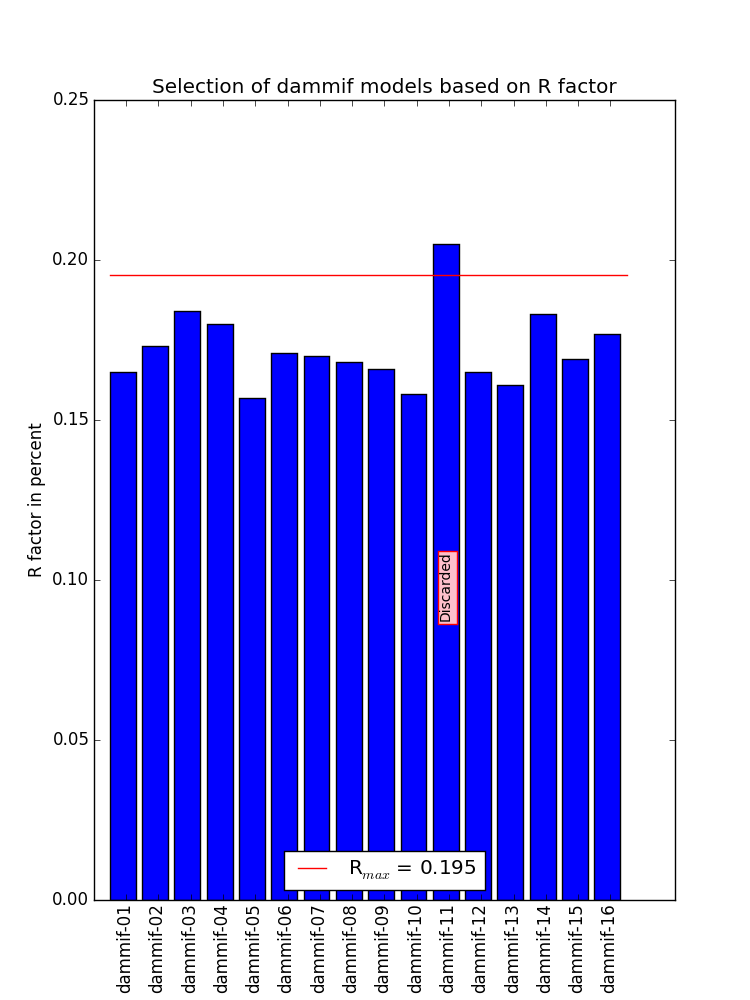
\includegraphics[scale=0.6]{Rfactor.png}
\caption{Graph containing the $R-value$ of each DAM, the maximal value 
         and the discarded DAM}
\label{fgr:rfactor}
\end{figure}
It points out the fact that the $R-value$ of one of the models (dammif-
11) exceed the $R_{max}$, which is the mean of the $R-values$ plus two 
times the standard deviation. 
The DAM dammif-11 is automatically flagged as non-valid and discarded. 
The model will not be take into account in the following of the 
\textit{SuPyComb} process, that will save execution time.\\
After all the process we detailled in chapter 2, \textit{SuPyComb} 
returns the two graphs presented in figure~\ref{fgr:nsd}. 
\begin{figure}
\centering
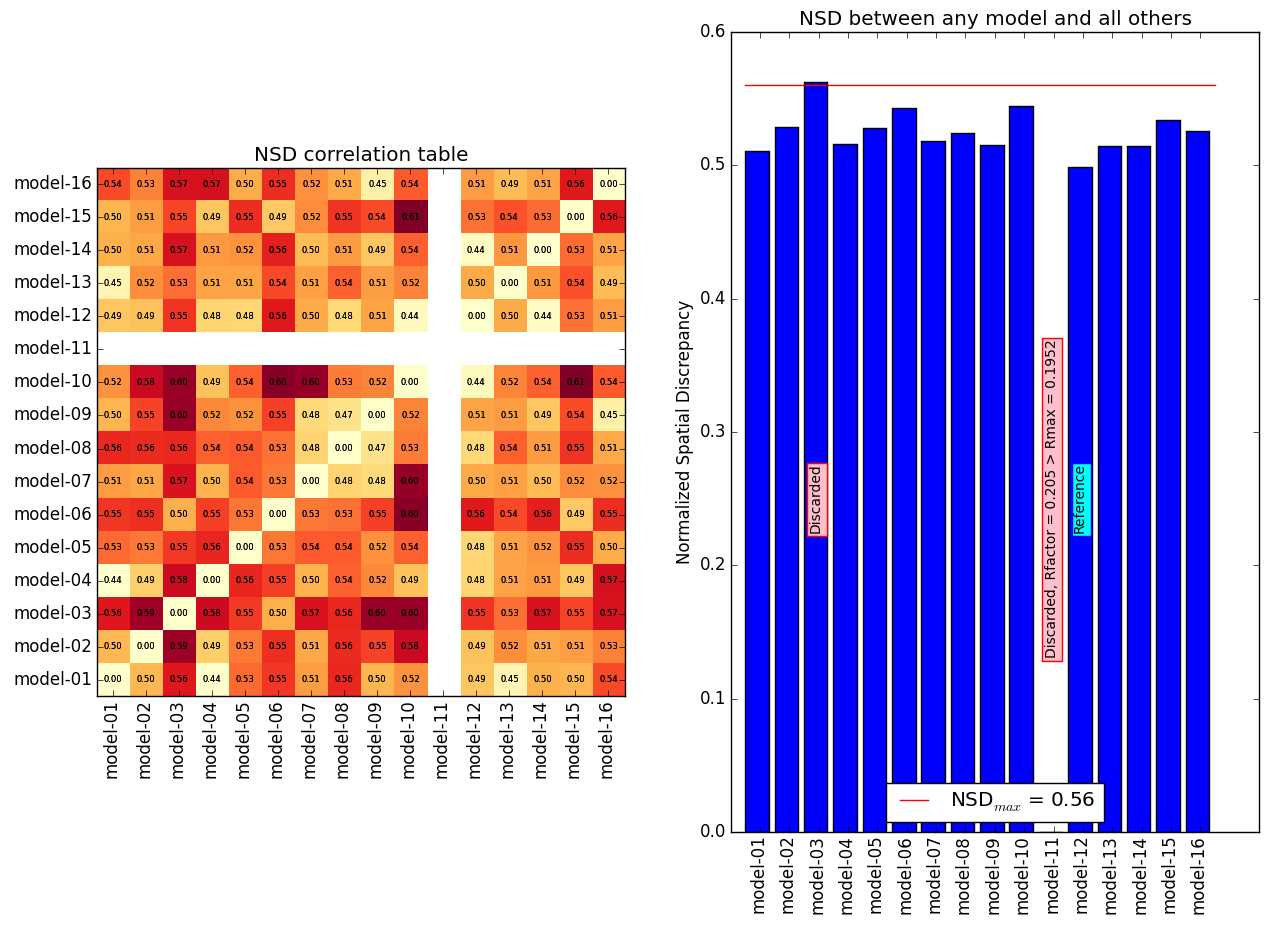
\includegraphics[scale=0.45]{nsd.png}
\caption{Two graphs computed by \textit{SuPyComb}, the NSD table and 
         the nsd mean with all other DAM for each model}
\label{fgr:nsd}
\end{figure}
The $16*16$ NSD table details the distance between each pair of 
models. 
The color scale accentuate the biggest and the lowest NSD values, 
which gives a clear idea of the similar models and the dis-similar 
ones.\\
The second graph ("NSD between any model and all others") give us 
five informations:
\begin{itemize}
\item as it is called, the NSD between any model and all others
\item the $NSD_{max}$ computed as the mean plus the standard deviation
\item the previously discarded models, and why they have been discarded
\item the models discarded due to their dis-similarity
\item the reference model, the one with the lowest value of NSD with 
      all other models
\end{itemize}
Here, the model "model-03" (which is the model "dammif-03" after 
translations and rotations) is flagged as non-valid.\\
Finally, remaining models (the ones flagged as valid) are superimpose 
on the reference model, here the DAM "model-12". 
The final positions of the 16 dummy-atoms models are then saved in 16 
pdb files, compatible with other \textsc{atsas} programs which may be 
ran.
%TODO mettre en annexes une representation des modeles valides avec Pymol
%avec une reference dans cette section ???

\section{SuPyComb's performances}%TODO titre definitif ?

Several sides of \textit{SuPyComb} make it interesting to use it in 
place of \textsc{atsas}'s \textit{supcomb}.

First, \textit{SuPyComb} is able to take as arguments several DAM 
whereas \textit{supcomb} only superimpose two models. 
Thus, for the superimposition of 16 models, it has to read several 
times each models (total of $16*16$ reading), whereas 
\textit{SuPyComb} reads only one time each pdb file.\\
Moreover, \textit{supcomb} do not generates graphs we need 
($R-values$, NSD table, NSD means), so it has to be done elsewhere. 
The fact that \textit{SuPyComb} generates it automatically simplify 
EDNA's run.\\
The execution time of \textit{SuPyComb} is also a great advantage 
comparatively to \textit{supcomb}. 
Some tests has been performed to compare execution times with several 
option of both programs (always with the same SAXS curve of the 
Lysozyme protein). 
Results are presented in the appendix.\\%TODO ajouter reference et commentaires
Can be added to these advantages the fact, already mentionned, that a 
Python implementation provides a better integration into EDNA 
pipeline.\\

We saw in this chapter that FreeSAS provides tools to analyse and 
handle effectively data from \textit{dammif}. 
\textit{SuPyComb} program from FreeSAS returns good results, that are 
compatible with others \textsc{atsas} programs used into EDNA.


\chapter*{Conclusion and outlook}
\addcontentsline{toc}{chapter}{Conclusion and outlook}
    %----------------------------------------
    % Chapitre de conclusion + perspectives
    %----------------------------------------


\newpage                 %ne pas enlever (numerotation pour sommaire)
\addcontentsline{toc}{chapter}{Bibliography}
\bibliographystyle{plain}%ou autre ???
\bibliography{bibliography}
    %-------------------------
    % Bibliographie du stage
    %-------------------------


\appendix
    %---------------------
    % Annexes du rapport
    %---------------------

%a voir pour le contenu

\chapter{First appendix}

\chapter{Second appendix}


\end{document}

